\documentclass[11.5pt]{sig-alternate} % sets document style to sig-alternate
% packages
% typesetting
%\usepackage{dirtytalk} % typset quotations easier (\say{stuff})
\usepackage{hanging} % hanging paragraphs
\usepackage[defaultlines=3,all]{nowidow} % avoid widows
\usepackage[pdfpagelabels=false]{hyperref} % produce hypertext links, includes backref and nameref
\usepackage{xurl} % defines url linebreaks, loads url package
\usepackage{microtype}
\usepackage{textgreek}
%\usepackage{textcomp}
%\newcommand{\texttildemid}{\raisebox{0.4ex}{\texttildelow}}
% layout
\usepackage{enumitem} % control layout of itemize, enumerate, description
\usepackage{fancyhdr} % control page headers and footers
\usepackage{float} % improved interface for floating objects
%\usepackage{multicol} % intermix single and multiple column pages
% language
\usepackage[utf8]{inputenc} % accept different input encodings
\usepackage[english]{babel} % multilanguage support
% misc
\usepackage{graphicx} % builds upon graphics package, \includegraphics
%\usepackage{lastpage} % reference number of pages
%\usepackage{comment} % exclude portions of text (?)
\usepackage{xcolor} % color extensions
\usepackage[backend=biber, style=apa]{biblatex} % sophisticated bibliographies % necessary for HTML to display author info and date on abstract page
\usepackage{csquotes} % advanced quotations, makes biblatex happy
\usepackage{authblk} % support for footnote style author/affiliation
% tables and figures
\usepackage{tabularray}
%\usepackage{array} % extend array and tabular environments
\usepackage{caption} % customize captions in figures and tables (rotating captions, sideways captions, etc)
%\usepackage{cuted} % allow mixing of \onecolumn and \twocolumn on same page
\usepackage{multirow} % create tabular cells spanning multiple rows
%\usepackage{subfigure} % deprecated, support for manipulation of small figures
%\usepackage{tabularx} % extension of tabular with column designator "x", creates paragraph-like column whose width automatically expands
%\usepackage{wrapfig} % allows figures or tables to have text wrapped around them
%\usepackage{booktabs} % better rules
% dummy text
%\usepackage{blindtext} % blind text dummy text
%\usepackage{kantlipsum} % Kant style dummy text
\usepackage{lipsum} %lorem ipsum dummy text
% other helpful packages may be booktabs, longtable, longtabu, microtype

\pagestyle{fancy} % sets pagestyle to fancy for fancy headers and footers

% header and footer
% modern way to set header image
\renewcommand{\headrulewidth}{0pt} % defines thickness of line under header
\renewcommand{\footrulewidth}{0pt} % defines thickness of line above header
\setlength\headheight{80.0pt} % sets height between top margin and header image, effectively moves page contents down
\addtolength{\textheight}{-80.0pt} % seems to affect the lower height. maybe only works properly if footer numbers enabled?
\fancyhf{}
\fancyhead[CE, CO]{
\includegraphics[width=\textwidth]{headerImage.png}}
% footer
%\fancyfoot[LE,LO]{Article Title Here \\ DOI: }% left footer article title and doi
%\fancyfoot[CE,CO]{{}} % center footer empty
%\fancyfoot[RE,RO]{\thepage} % right footer page numbers
%\pagenumbering{arabic} % arabic (1, 2, 3) numbering in footer

\hypersetup{colorlinks=true,urlcolor=blue} % sets link color to blue
\urlstyle{same} % sets url typeface to same as rest of text

% set caption and figure to italics, label bold, left align captions, does not transfer to HTML
\captionsetup{labelfont=bf, font={large, it}, justification=raggedright, singlelinecheck=false}
\renewcommand\theContinuedFloat{\alph{ContinuedFloat}}

%this next bit is confusing, but essentially changes the width of the abstract. Seems to have been copied from this https://tex.stackexchange.com/questions/151583/how-to-adjust-the-width-of-abstract
\let\oldabstract\abstract
\let\oldendabstract\endabstract
\makeatletter %changes @ catcode to enable modification (in parsep)
\renewenvironment{abstract} %alters the abstract environment
{\renewenvironment{quotation}%
               {\list{}{\addtolength{\leftmargin}{1em} % change this value to add or remove length to the the default ?
                        \listparindent 1.5em%
                        \itemindent    \listparindent%
                        \rightmargin   \leftmargin%
                        \parsep        \z@ \@plus\p@}%
                \item\relax}%
               {\endlist}%
\oldabstract}
{\oldendabstract}
\makeatother %changes @ catcode to disable modification

% checks
% italics -
% links -
% dashes -
% tildes -
\begin{document}

\title{Using An Inquiry-based Teaching Approach to Improve Science Outcomes for Students with Disabilities: Snapshot and Longitudinal Data}

\author[1]{\large \color{blue} Jonte Taylor}
\author[1]{\large \color{blue} William J. Therrien}
\author[1]{\large \color{blue} Erica Rochelle Kaldenberg}
\author[1]{\large \color{blue} Sarah J. Watt}
\author[1]{\large \color{blue} Niphon Chanlen}
\author[1]{\large \color{blue} Brian Hand}


\affil[1]{The University of Iowa}
\toappear{}

\maketitle
\begin{@twocolumnfalse} 
\begin{abstract}
\item 
\begin{large}
\textit{Poor science achievement has been an educational issue for a number of years. Students with disabilities have traditionally fared worse. Research suggests that students with disabilities may respond better to instruction using an inquiry-based approach vs. traditional textbook instruction when measuring science achievement on standardized measures. The researchers report achievement data on the Iowa Test of Basic Skills from a target school district for students Individualized Education Program’s (IEP) and non-IEP students, as well as students with IEP’s at the state level. Using an argument-based inquiry approach to science instruction called the Science Writing Heuristic (SWH); the researchers report data supporting its impact on student achievement in science. Data suggest that the SWH may contribute to science achievement for students with IEP’s.}
\\ \\

\end{large}     
\end{abstract}
\end{@twocolumnfalse}

%% ABSTRACT

%% AUTHOR INFORMATION

\textbf{*Corresponding Author, Jonte Taylor}\\
\href{mailto:jonte-taylor@uiowa.edu}{(jonte-taylor@uiowa.edu)}\\
\textit{Submitted December 17, 2013}\\
\textit{Accepted December 17, 2013}\\
\textit{Published Online December 17, 2013}\\
\textit{DOI: 10.14448/jsesd.04.0003}\\

\pagebreak
\clearpage
\begin{large}
An increase in accountability for teachers and schools to ensure that students with disabilities are becoming proficient in the areas of reading, math, and science was promoted through the passing of No Child Left Behind (2002). This educational legislation, aligned closely with the Individuals with Disabilities Education Improvement Act (2004), has led to an increase in the number of students with disabilities receiving core science instruction in general education settings (Kirch, Bargerhuff, Cowan, \& Wheatly, 2007). As mandated by a student with disabilities Individualized Education Program (IEP), where and how a student receives educational support is an important consideration. Most students with disabilities spend at least 80\% of their day in general education. This change in inclusionary practices and an increased emphasis on science instruction and achievement has changed the focus of both general and special education teachers (Brigham, Scruggs, \& Mastropieri, 2011).

According to the National Educational Assessment Performance’s, National Center for Education Statistics (NCES, 2009) thirty-four percent of students at grade 4, some 30 percent of students at grade 8, and 21 percent of students at grade 12 performed at or above the \textit{Proficient} level in 2009. While there is an overall increase in the science achievement of students nationwide, students with disabilities are continuing to score significantly below their nondisabled peers. When analyzing these assessments, Thurlow, Rogers, and Christenson (2010) found that in 12 of 22 states, less than 50 percent of elementary students with disabilities attained proficiency or advanced levels of performance.

There are many reasons why students with disabilities may struggle in core science instruction. Difficulties with vocabulary knowledge and reading comprehension have been identified in research as learner characteristics that can cause great difficulty for students with disabilities (Therrien, Taylor, Hosp, Kaldenberg, \& Gorsh, 2011). Traditional science instruction relies heavily on teaching content through lecture and the use of a science textbook (Brigham, Scruggs, \& Mastropieri, 2011). Often students do not receive the instruction necessary to promote strong understanding and comprehension of expository text that is laced with complex vocabulary and an expectation that the student has prior knowledge in the subject area (Mason \& Hedin, 2011). As a result students with these characteristics become frustrated and unmotivated to do well in science class. Both students with and without disabilities are faced with this challenge in core science instruction. Other characteristics of students with disabilities that can impede science performance are difficulties in math, processing and retaining information, attention-deficits, and inappropriate classroom behavior.

Research has shown that one way to minimize the challenges that students with disabilities face in the science classroom is to instruct using an inquiry-based approach vs. traditional textbook instruction (Scruggs, Mastropieri, Bakken, \& Brigham, 1993). The reform efforts of many national science organizations over the last decade have endorsed this approach as a means of focusing on the depth of learning vs. the breadth of traditional curriculum frameworks. This hands-on approach to learning allows students to engage in and discover core concepts by conducting experiments and making connections through problem solving and negotiation. Inquiry-based instruction focuses on big ideas versus rote memorization of facts which helps students to retain information they learn more easily. Focusing on core concepts can encourage students to extend their learning beyond traditional science lessons and instruction.

The purpose of this article is to provide descriptive data associated with the learning gains the authors contend correlates with the Science Writing Heuristic in the area of science education for students with disabilities. The researchers used data supplied by the target school district for a “snapshot” analysis of science achievement for one school year and data supplied by the state department of education to determine longitudinal outcomes.

\section*{METHOD}
\subsection*{Participants}
The target school district in this study is located in a rural area of a Midwestern state. The students included in this study were those who participated in general education science classes. The students with disabilities in the study were identified as students with IEP’s using the information provided by the state assessment for progress monitoring, the Iowa Test of Basic Skills (ITBS) for the school year of 2009-2010 (see Table 1). A subset of 23 students with disabilities were tracked beginning in 2006 (3rd grade) through 2011 (8th grade). \\

\subsection*{Procedure}
Science teachers in the target school district were introduced to the Science Writing Heuristic (SWH) as a means of teaching science content and method to students. The teachers at the target school district began using the SWH instructional approach in 2000 initially in 6th-10th grades. After two years of teacher reported and standardized tests success in science, teachers in elementary grades (3rd-5th) began using the SWH procedure and methodology. In 2005, teachers in kindergarten through 2nd grades were introduced to the SWH approach. Science teachers in the target school district now use the SWH approach district-wide.

\subsection*{Intervention}
\textit{The science writing heuristic.} The Science Writing Heuristic (SWH) is an argument-based inquiry approach that has demonstrated success in terms of both teacher implementation and student achievement (Hand \& Keys, 1999). The SWH approach is designed to involve students in inquiry, argumentation, and experimentation as a means of learning science and improving critical thinking skills. Based on the theories that include writing-to-learn strategies, science literacy, and inquiry-based instruction (Yore, Bisanz, \& Hand, 2003), the SWH approach was developed as a means of providing students a conceptual framework for science knowledge through debate and experimentation while simultaneously allowing for multiple means of expression to display robust understanding of science themes and concepts. Developed by Brian Hand and Carolyn Keys in the late 1990’s, the SWH requires students to use “questions, claims, and evidence” to display understanding of science content and concepts.

\begin{table*}[th]
\caption{Target School District Participation on the Iowa Test of Basic Skills (2009-2010)*}
\begin{tabular}{lcccccccc}
\hline
Students & 3rd Grade & 4th Grade & 5th Grade & 6th Grade & 7th Grade & 8th Grade & 11th Grade & Total \\ \hline
\multicolumn{9}{l}{Participation - Number}\\ \hline
non-IEP & 135 & 163 & 144 & 175 & 183 & 358 & 164 & 1547 \\
IEP & 21 & 20 & 28 & 28 & 38 & 66 & 24 & 225 \\ \hline
\multicolumn{9}{l}{Participation – Percentages} \\ \hline
non-IEP & 87\% & 89\% & 84\% & 86\% & 83\% & 84\% & 87\% & 85\%  \\
IEP & 13\% & 11\% & 16\% & 14\% & 17\% & 16\% & 13\% & 15\%  \\ \hline
\end{tabular}
Note- The data show participation rate for the target school district. The target school district is classified as a rural population area in a Midwestern state.
\end{table*}

The SWH is grounded in the idea that people are active in their own learning or knowledge construction (Strike, 1987). The National Science Education Standards place great emphasis on the need for students to be active learners, to inquire and be curious about science, and to communicate their understandings to others. Specifically, the SWH concentrates on broad conceptual understanding, concept maps, and student argumentation and negotiation to encourage students to connect science practically.

\textit{Inquiry-based instruction and hands-on experimentation.} As recommended by the National Research Council (1996), the SWH emphasizes the use of inquiry-based instruction. Unfortunately, there has been no general consensus of exactly what constitutes inquiry-based instruction (Klahr \& Li, 2005; Minner, Levy, \& Century, 2010). Scruggs and Mastropieri (2007) explain that inquiry-based instruction builds concept knowledge and learning depth of science content. In addition to inquiry-based instruction, the use of hands-on experimentation and structure is recommended for students with disabilities (Scruggs, Mastropieri, \& Boon, 1998). The SWH uses student directed practices with teacher guidance and the opportunity for students to conduct experiments of their own devices. Students are required to develop their own research questions, create a claim, and conduct experiments to support or reject their claims.

\textit{SWH templates.} Scruggs and Mastropieri (2007) suggest that inquiry-based instruction should include an intensive level of structure for students with disabilities. The SWH uses teacher and student templates to scaffold the teaching and learning process during science instruction (see Table 2). The teacher template addresses teacher activities as they relate to the SWH approach. In the teacher template, the teachers are directed to use a series of strategies connected to the identified elements of the SWH. The template encourages teachers to provide students with multiple opportunities to negotiate understanding of science concepts through their own ideas and experiences. The purpose of the teacher template is to provide instructional guides for pedagogical support of student learning. The student template serves to scaffold student understanding of scientific concepts while at the same time emphasizing the processes of scientists. The SWH encourages students to understand the way in which science is conducted through research, experimentation, negotiation of ideas, refinement of ideas, and explanations of conclusions.

\subsection*{Measure}
\textit{The Iowa Test of Basic Skills.} The Iowa Test of Basic Skills (ITBS) consists of a battery of achievement subtests that is used to assess student performance in specific content areas. The ITBS is used to provide achievement information for teachers that in turn can be used to help improve instruction and provide information regarding student learning trends. Additionally, the ITBS is used as an accountability measure by a number of states. Schools are required to have a certain percentage of students reach “proficient” which indicates acceptable demonstration of academic knowledge. Proficiency percentages are reported by the state and by each school district who participates.

The ITBS was used by the target school district to assess students’ achievement and to make academic decisions regarding student educational programming. For the purposes of the current study, the ITBS subtests of reading comprehension, math, and science were examined. Particular attention was paid to the science subtest which assesses scientific inquiry, life science, earth/space science, and physical science (for additional information regarding the ITBS see \url{http://www.riverpub.com/products/itbs/index.html}).

\begin{table*}[thp]
\caption{Student and Teacher Template for the Science Writing Heuristic approach}
\begin{tabular}{lll}
\hline
\textbf{Student Template} & & \textbf{Teacher Template} \\ \hline
1. Beginning Ideas & What are my questions? & Exploration of pre-instruction understanding through individual or group concept mapping or working through a computer simulation. \\ \hline
2. Tests & What did I do? & Pre-laboratory activities, including informal writing, making observations, brainstorming, and posing questions. \\ \hline
3. Observations & What did I see? & Participation in laboratory activity. \\ \hline
4. Claims & What can I claim? & Negotiation phase I - writing personal meanings for laboratory activity. \\ \hline
5. Evidence & How do I know? How can I support my claim & Negotiation phase II - sharing and comparing data interpretations in small groups. \\ \hline
6. Reading & How do my ideas compare with others ideas? & Negotiation phase III - comparing science ideas to textbooks for other printed resources. \\ \hline
7. Reflection & How have my ideas changed? & Negotiation phase IV - individual reflection and writing. \\ \hline
8. Writing & What is the best explanation to describe what I have learned? & Exploration of post-instruction understanding through concept mapping, group discussion, or writing a clear explanation. \\ \hline
\end{tabular}
\end{table*}

\subsection*{Calculations}
Proficiency percentages are reported by the state and by each school district who participates. The authors used the reported percentages to conduct comparisons. The proficiency differences were calculated by subtracting science proficiency percentages from the proficiency percentages in the areas of reading comprehension and math respectively.

\section*{RESULTS}
The results are presented by the researchers examining comparisons between students with IEP’s from the target school district, non-IEP students from the target school district, and students with IEP’s statewide, produced from Iowa Test of Basic Skills (ITBS) data. The following comparisons were made: 
\begin{enumerate}[label=(\alph*)]
    \item proficiency percentages during one academic school year (2009-2010) for students with Individualized Education Plans (IEP) in grades 3 through 8 and grade 11 on the ITBS subtests of science, math, and reading comprehension at the target school district;
    \item proficiency percentages for students with IEP’s from the target school district versus those at the state level on the ITBS science subtest;
    \item proficiency percentage differences between science and reading comprehension subtests and science and math subtests respectively for students with IEP’s versus non-IEP students at the target school district;
    \item proficiency percentage differences between science and reading comprehension subscales and science and math subscales respectively for students with IEP’s from the target school district versus those at the state level; and
    \item longitudinal proficiency percentages on the ITBS science subtest and improvement difference percentages on science and reading comprehension and science and math subtests respectfully for students with IEP’s at the target school district versus students with IEP’s at the state level from the years of 2006 to 2011.
\end{enumerate}

\begin{figure*}
    \centering
    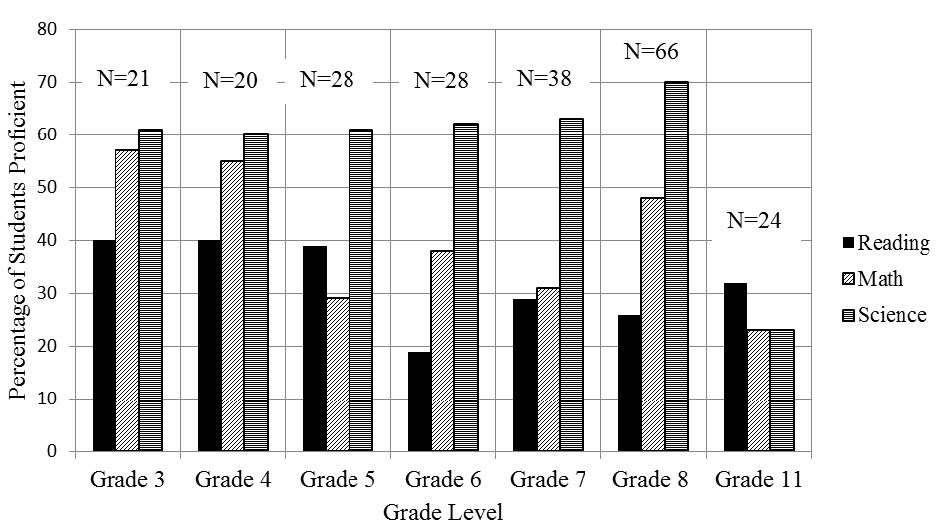
\includegraphics{Figure 1.jpg}
    \caption{Proficiency Percentages for Students with IEP's on the Iowa Test of Basic Skills}
    \label{fig:Figure 1}
\end{figure*}

\subsection*{2009-2010 Proficiency Data}
\textit{Proficiency percentages.} During the 2009-2010 school year, approximately 15\% of students with IEP’s participated in ITBS from grades 3-8 and grade 11 (see Table 2). Scores for grades 9 and 10 were not available. In all grades, with the exception of grade 11, proficiency in science for students with IEP’s was higher than reported proficiency in reading and math. Proficiency percentage results ranged from approximately 19\%-40\%, 23\%-55\%, and 23\%-70\% on reading comprehension, math, and science subscale scores respectively (\textit{see Figure 1}). When compared to students with IEP’s at the state level, the target school district reached higher levels of proficiency on the ITBS science subtest. Approximately 50\% students with IEP’s at the state level reached proficiency compared to 63\% at the target school district.

\textit{Proficiency percentage differences.} Difference comparisons of ITBS subtests science/reading comprehension and science/math at the target school district revealed that students with IEP’s had higher improvement differences in proficiency versus non-IEP students in most instances (\textit{see Table 3}). Examination of fourteen comparisons (7 science/reading comprehension and 7 science/math, respectively) resulted in only four instances of non-IEP students showing better improvement than students with IEP’s from the target school district. Students with IEP’s at the target school district had slightly higher proficiency percentage differences on the ITBS compared to students with IEP’s at the state level for the 2009-2010 school year (see Figure 2).

\begin{figure}[t]
    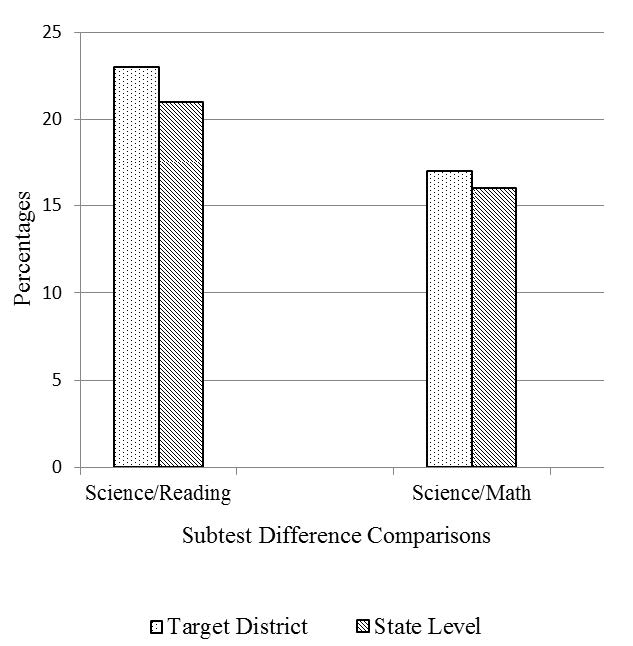
\includegraphics[width=\columnwidth]{Figure 2.jpg}
    \caption{\textit{Proficiency Percentage Differences for Students with IEP’s on the Iowa Test of Basic Skills. Percentage differences of the ITBS subtest of science and reading comprehension and science and math. Comparisons are of students with IEP’s at the target district and state levels.}}
    \label{Figure 2}
\end{figure}

\subsection*{2006-2011 Longitudinal Data}
\textit{Proficiency percentages.} Longitudinal data on students with IEP’s entering third grade in 2006 through eighth grade in 2011 were examined from the target school district and compared with students with IEP’s at state level for each of respective year. These data showed that the tracked students at the target school district reached higher proficiency percentages on the ITBS science subtest in all but years 2008 and 2009 respectively compared to students with IEP’s at the state level (see Figure 3). When comparing proficiency improvement differences, these data showed similar results (see Table 4). For most comparisons, the target school district showed higher levels of improvement than students at the state level. The authors noted that science/reading comprehension improvements for the students with IEP’s at the target school district were lower than those at the state level for the year of 2007. It should also be noted that while examining the data for 2008, the students in the target school district showed no improvement differences when compared to state level percentages. There were no data available for students in the target school district for the year of 2009 due to changes in reporting by building (e.g. students in grades 6 were moved from elementary school to middle school).

\begin{figure}[t]
    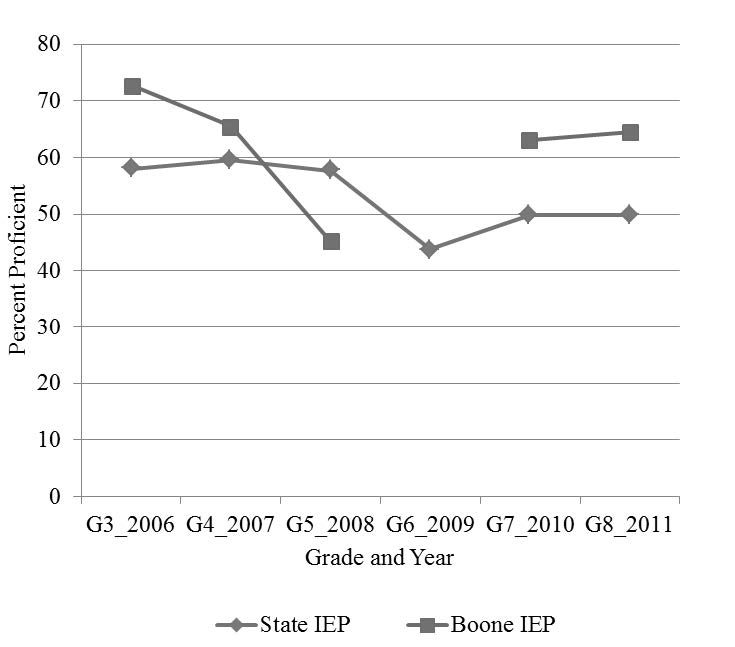
\includegraphics[width=\columnwidth]{Figure 3.jpg}
 \caption{\textit{Longitudinal Proficiency Percentages for Students with IEP’s on the Iowa Test of Basic Skills Science Subtest. Longitudinal Proficiency Percentages on the ITBS science subtest Comparisons are of students with IEP’s at the target district and state levels for the years of (2006-2011). Note-The school district did not provide data for the 2009 school year.}}
\end{figure}

\section*{DISCUSSION}
The purpose of this article was to examine the impact of SWH approach for students with disabilities. Using a one year “snapshot” of students and 23 students tracked over a six year period, comparisons were made between the non-IEP students from the target school district and students with IEP’s statewide. The ITBS scores were analyzed and the percentage of students proficient in the areas of reading comprehension, math, and science were compared.

Within group comparisons of students with IEP’s at the target school district showed that students were generally more proficient in science than other subtest areas during the snapshot year. Also during the single year examination, when compared with students with IEP’s at the state level, the students in the target school district reached a substantially higher proficiency percentage. These results suggest that the science program in the target school district may lead to a higher percentage of students with IEPs scoring proficient on the ITBS science subtest compared to the percentage of students with IEPs who also score proficient across the state during one academic year. Results from longitudinal comparisons of students with IEP’s, ITBS science subtest proficiency percentages suggest equally impressive science achievement results. After tracking twenty-three students for six years, all but two years displayed students with IEP’s at the target school district reaching higher proficiency on the ITBS science subtest when compared to students with IEP’s at the state level. During the final two years of tracking, 2010 (7th grade) and 2011 (8th grade) respectively, students at the target district reached substantially higher proficiencies compared to students at the state level.

When looking at the science program in this district, we know the science teachers were trained to use and implement the SWH approach. Although, we cannot say for certain that the SWH model is the reason why we are seeing the trend, we do know that there are many components used within SWH that researchers suggest produce higher results for students with special needs.

\begin{table*}[tph]
\caption{2009-2010 School Year Data Proficiency Percentage Differences for Target School District}
\begin{tabular}{lllll}
\hline
 & \multicolumn{2}{l}{Science/Reading} & \multicolumn{2}{l}{Science/Math} \\ \hline
Grade & non-IEP & IEP & non-IEP & IEP \\ \hline
3rd & -3\% & 21\% & 6\% & 4\% \\
4th & 0\% & 20\% & -1\% & 5\% \\
5th & 5\% & 5\% & 22\% & 32\% \\
6th & 23\% & 43\% & 13\% & 24\% \\
7th & 8\% & 34\% & 17\% & 32\% \\
8th & 16\% & 44\% & 7\% & 22\% \\
11th & 5\% & -9\% & 0\% & 0\% \\ \hline
\end{tabular}
\end{table*}

\begin{table*}[tph]
\caption{Longitudinal Data on Proficiency Percentage Differences for Students with IEP’s}
\begin{tabular}{lllll}
\hline
 & \multicolumn{2}{l}{Target School District} & \multicolumn{2}{l}{State Level} \\ \hline
Year & Science/Reading & Science/Math & Science/Reading & Science/Math \\ \hline
2006 & 32\% & 30\% & 23\% & 13\% \\
2007 & 9\%\textsuperscript{a} & 13\% & 18\% & 10\% \\
2008 & -10\%\textsuperscript{ab} & 0\%\textsuperscript{ab} & 20\% & 12\% \\
2009 & N/A\textsuperscript{c} & N/A\textsuperscript{c} & 16\% & 9\% \\
2010 & 35\% & 33\% & 23\% & 16\% \\
2011 & 32\% & 17\% & 21\% & 15\% \\ \hline
\end{tabular}
\textsuperscript{a}Indicates areas in which science comparisons were larger for state than target school district.

\textsuperscript{b}Indicates areas when there were either no change or no improvement in proficiency difference.

\textsuperscript{c}N/A=Not Available. Proficiency percentages were not available for that school year.

\end{table*}

\section*{INFLUENTIAL COMPONENTS}
For the 23 students with special needs, science instruction was delivered using an inquiry method —specifically following the SWH model; and we know that students with special needs can be successful in such inquiry-based classes (Mastropieri \& Scruggs, 1992; Mastropieri et al., 1998). Researchers also suggest it may be specific components of the SWH inquiry model that that are contributing to this success. One of these major components of a SWH classroom is the movement away from providing instruction using a textbook. The complex text and vocabulary often associated with science textbooks is often a barrier to students with learning difficulties (Parmar, Duluca, \& Janczak, 1994). Secondly in SWH classrooms, textbooks are replaced by hands on-concrete experiences. In a meta-analysis of science instruction for students with LD, Therrien, et al., (2011) concluded that students seem to benefit from these types of classroom activities. Another unique characteristic of the SWH approach, which research has shown to help students with disabilities, is that the learning experiences are geared around big ideas. In the same meta-analysis for students with LD, Therrien and colleagues (2011) found that intervention studies for students with LD in the content area of science that focused on big ideas by using graphic organizers produced a larger effect size (ES) than studies that did not.

\subsection*{Limitations}
There are a few major limitations to the conclusions of this study. First, although the teachers in this school district received extensive training on how to successfully implement this approach in their classrooms along with constructive feedback to improve their use of the model, results of the study are limited by lack of teaching fidelity data.

Secondly, the Midwest state where this study took place does not follow the traditional model of identification of students with special needs. This state classifies all students who receive services under an IEP as an eligible individual not as a student with a particular disability. This classification system makes it impossible to further explore the efficacy of the SWH approach on students with varying disabilities (e.g., students with learning disabilities, students with intellectual disabilities, student with emotional and behavior disabilities, etc.). Third, comparisons made here were based on extant data, with no real control group available at the student and school levels. Additional studies that examine the impact of the SWH using experimental designs (e.g., random control trial) need to be conducted before we can ascertain with certainty the effectiveness of the SWH on students with disabilities science achievement. Furthermore, the study data regarding participants at both the snapshot and longitudinal levels are consistent with rural population data. As the target school district was a rural population area in a Midwestern state inferences based on study results should be limited to the similar population demographics.

\section*{CONCLUSION}
Overall results indicate that the SWH approach for teaching science to students with disabilities has the potential to be effective at increasing students with disabilities achievement on the ITBS assessment. This coincides with past research, which suggested that students with disabilities can be successful in inquiry classrooms. However, research also suggests that such students may be even more successful if they receive significantly more structure (Dalton et al. 1997; McCleery and Tindal, 1999). As previous literature reviews tend to suggest (Mastropieri \& Scruggs, 1992; Scruggs, Mastropieri, \& Boon, 1998), future research in SWH classrooms should focus on providing students with disabilities additional support such as pre-teaching important concepts, modifying or adapting language requirements, supporting hands-on experiences and providing formative feedback.

\textit{The research reported here was supported by the Institute of Education Sciences, U.S. Department of Education, through Grant R305B10005 to The University of Iowa. The opinions expressed are those of the authors and do not represent views of the Institute or the U.S. Department of Education.}

\section*{BIOGRAPHICAL STATEMENTS}
\textbf{Jonte C. Taylor} (\href{mailto:jonte-taylor@uiowa.edu}{jonte-taylor@uiowa.edu}) is a postdoctoral scholar at the University of Iowa. His research interests include science instruction for students with mild cognitive disabilities, task engagement, bullying, and innovative instructional methods.

\textbf{William J. Therrien} (\href{mailto:bill-therrien@uiowa.edu}{bill-therrien@uiowa.edu}) is an associate professor and co-director of the Center for Disability Research and Education at the University of Iowa. His current research interests include science and reading instruction for students with learning disabilities.

\textbf{Erica R. Kaldenberg} (\href{mailto:erica-kaldenberg@uiowa.edu}{erica-kaldenberg@uiowa.edu}) is a doctoral student at the University of Iowa. Her research interests include science and writing instruction for students with disabilities.

\textbf{Sarah Watt} (\href{mailto:sarah-watt@uiowa.edu}{sarah-watt@uiowa.edu}) is a doctoral student at the University of Iowa. Her research interestes include Tier 2 math, reading, and science interventions for students with learning and behavioral disabilities.

\textbf{Niphon Chanlen} (\href{mailto:niphon.chanlen@uiowa.edu}{niphon.chanlen@uiowa.edu}) is a doctoral student in science education at the University of Iowa . His research of interest is professional development in science literacy.

\textbf{Brian Hand} (\href{mailto:brian-hand@uiowa.edu}{brian-hand@uiowa.edu}), Professor of Science Education has a research interest in emaining how language can be used to help promote student learning. He is particularly interested in how language use can be improved through science argumentative practices. 

\end{large}
\clearpage
\section*{REFERENCES}\par 

\leftskip 0.25in
\parindent -0.25in 
%%%
Bakken, J. P., Mastropieri, M. A., \& Scruggs, T. E. (1997). Reading comprehension of expository science material and students with learning disabilities: A comparison of strategies. Journal of Special Education, 31(3), 300-24.

Brigham, F. J., Scruggs, T. E., \& Mastropieri, M. A. (2011). Science education and students with learning disabilities. Learning Disabilities Research \& Practice, 26(4), 223-232.

Dalton, B., Morocco, C. C., Tivnan, T., \& Rawson Mead, P. L. (1997). Supported inquiry science: Teaching for conceptual change in urban and suburban science classrooms. Journal of Learning Disabilities, 30, 670–684

Hand, B., \& Keys, C. (1999). Inquiry investigation: A new approach to laboratory reports. The Science Teacher, 66, 27-29.

Individuals with Disabilities Education Improvement Act of 2004, Pub. L. No. 108-446. (2004). Retrieved from \url{http://idea.ed.gov/download/statute.html}

Kirch, S. A., Bargerhuff, M. E., Cowan, H., \& Wheatly, M. (2007). Reflections of educators in pursuit of inclusive science classrooms. Journal of Science Teacher Education, 18(4), 663-692.

Klahr, D. \& Li, J. (2005). Cognitive research and elementary science instruction: From the laboratory, to the classroom, and back. Journal of Science Education and Technology, 14(2), 217-238. doi: 10.1007/s10956-005-4423-5

Mason, L. H., \& Hedin, L. R. (2011). Reading science text: Challenges for students with learning disabilities and considerations for teachers. Learning Disabilities Research \& Practice, 26(4), 214-222.

Mastropieri, M. A., \& Scruggs, T. E. (1992). Science for students with disabilities. Review of Educational Research, 62, 377–411.

Mastropieri, M. A., Scruggs, T. E., Mantzicopoulous, P., Sturgeon, A., Goodwin, L., \& Chung, S. (1998). “A place where living things affect and depend on each other”: Qualitative and quantitative outcomes associated with inclusive science teaching. Science Education, 82, 163–179.

McCleery, J. A., \& Tindal, G. A. (1999). Teaching the scientific method to at-risk students and students with learning disabilities through concept anchoring and explicit instruction. Remedial and Special Education, 20, 7–18.

Minner, D. D., Levy, A. J., \& Century, J. (2010). Inquiry-based science instruction—what is it and does it matter? Results from a research synthesis years 1984 to 2002. Journal of Research In Science Teaching, 47(4), 474-496. doi: 10.1002/tea.20347

National Center for Education Statistics. (2011). The Nation’s Report Card: Science 2009 (NCES 2011-451). Institute of Education Sciences, U.S. Department of Education, Washington, D.C. Retrieved from \url{http://nces.ed.gov/nationsreportcard/pdf/main2009/2011451.pdf}

National Research Council (NRC) (1996). National Science Education Standards. Washington, DC: National Academy Press.

No Child Left Behind (NCLB) Act of 2001, Pub. L. No. 107-110, § 115, Stat. 1425 (2002).

Parmar, R. S., Deluca, D. B., \& Janczak, T. M. (1994). Investigations into the relationship between science and language abilities of students with mild disabilities. Remedial and Special Education, 15, 117–126.

Scruggs, T. E., \& Mastropieri, M. A. (2007). Science learning in special education: The case for constructed versus instructed learning. Exceptionality, 15, 57-74. doi:10.1080/09362830701294144

Scruggs, T. E., Mastropieri, M. A., Bakken, J. P., \& Brigham, F. J. (1993). Reading versus doing: The relative effects of textbook-based and inquiry-oriented approaches to science learning in special education classrooms. Journal of Special Education, 27, 1-15. doi:10.1177/00224669930270010

Scruggs, T. E., Mastropieri, M. A., \& Boon, R. (1998). Science education for students with disabilities: A review of recent research. Studies in Science Education, 32, 21–44.

Strike, K. A. (1997). Toward a coherent constructivism. In J. Novak (Ed.), Proceedings of the 2nd International Seminar Misconceptions and Educational Strategies in Science and Mathematics, Vol. 1. Ithaca, NY: Cornell University, 481-489.

Therrien, W. J., Taylor, J. C., Hosp, J. L., Kaldenberg, E. R., \& Gorsh, J. (2011). Science instruction for students with learning disabilities: A meta-analysis. Learning Disabilities Research \& Practice, 26(4), 188-203.

Thurlow, M., Rogers, C., \& Christenson, L. (2010). Science assessment for students with disabilities in school year 2006–2007: What we know about participation, performance, and accommodations (Synthesis Report 77). Minneapolis, MN: University of Minnesota, National Center for Educational Outcomes.

Yore, L. D., Bisanz, G. L., \& Hand, B. M. (2003). Examining the literacy component of science literacy: 25 years of language arts and science research. International Journal of Science Education, 25, 689-725.


\end{document}
